\documentclass[a4paper, 12pt, garamond]{book}
\usepackage{cours-preambule}

\setlength{\mtcindent}{-10pt}
\mtcsetoffset{minitoc}{-10pt}

\begin{document}

\begin{adjustwidth}{-1cm}{-1cm}
	\pagestyle{empty}
	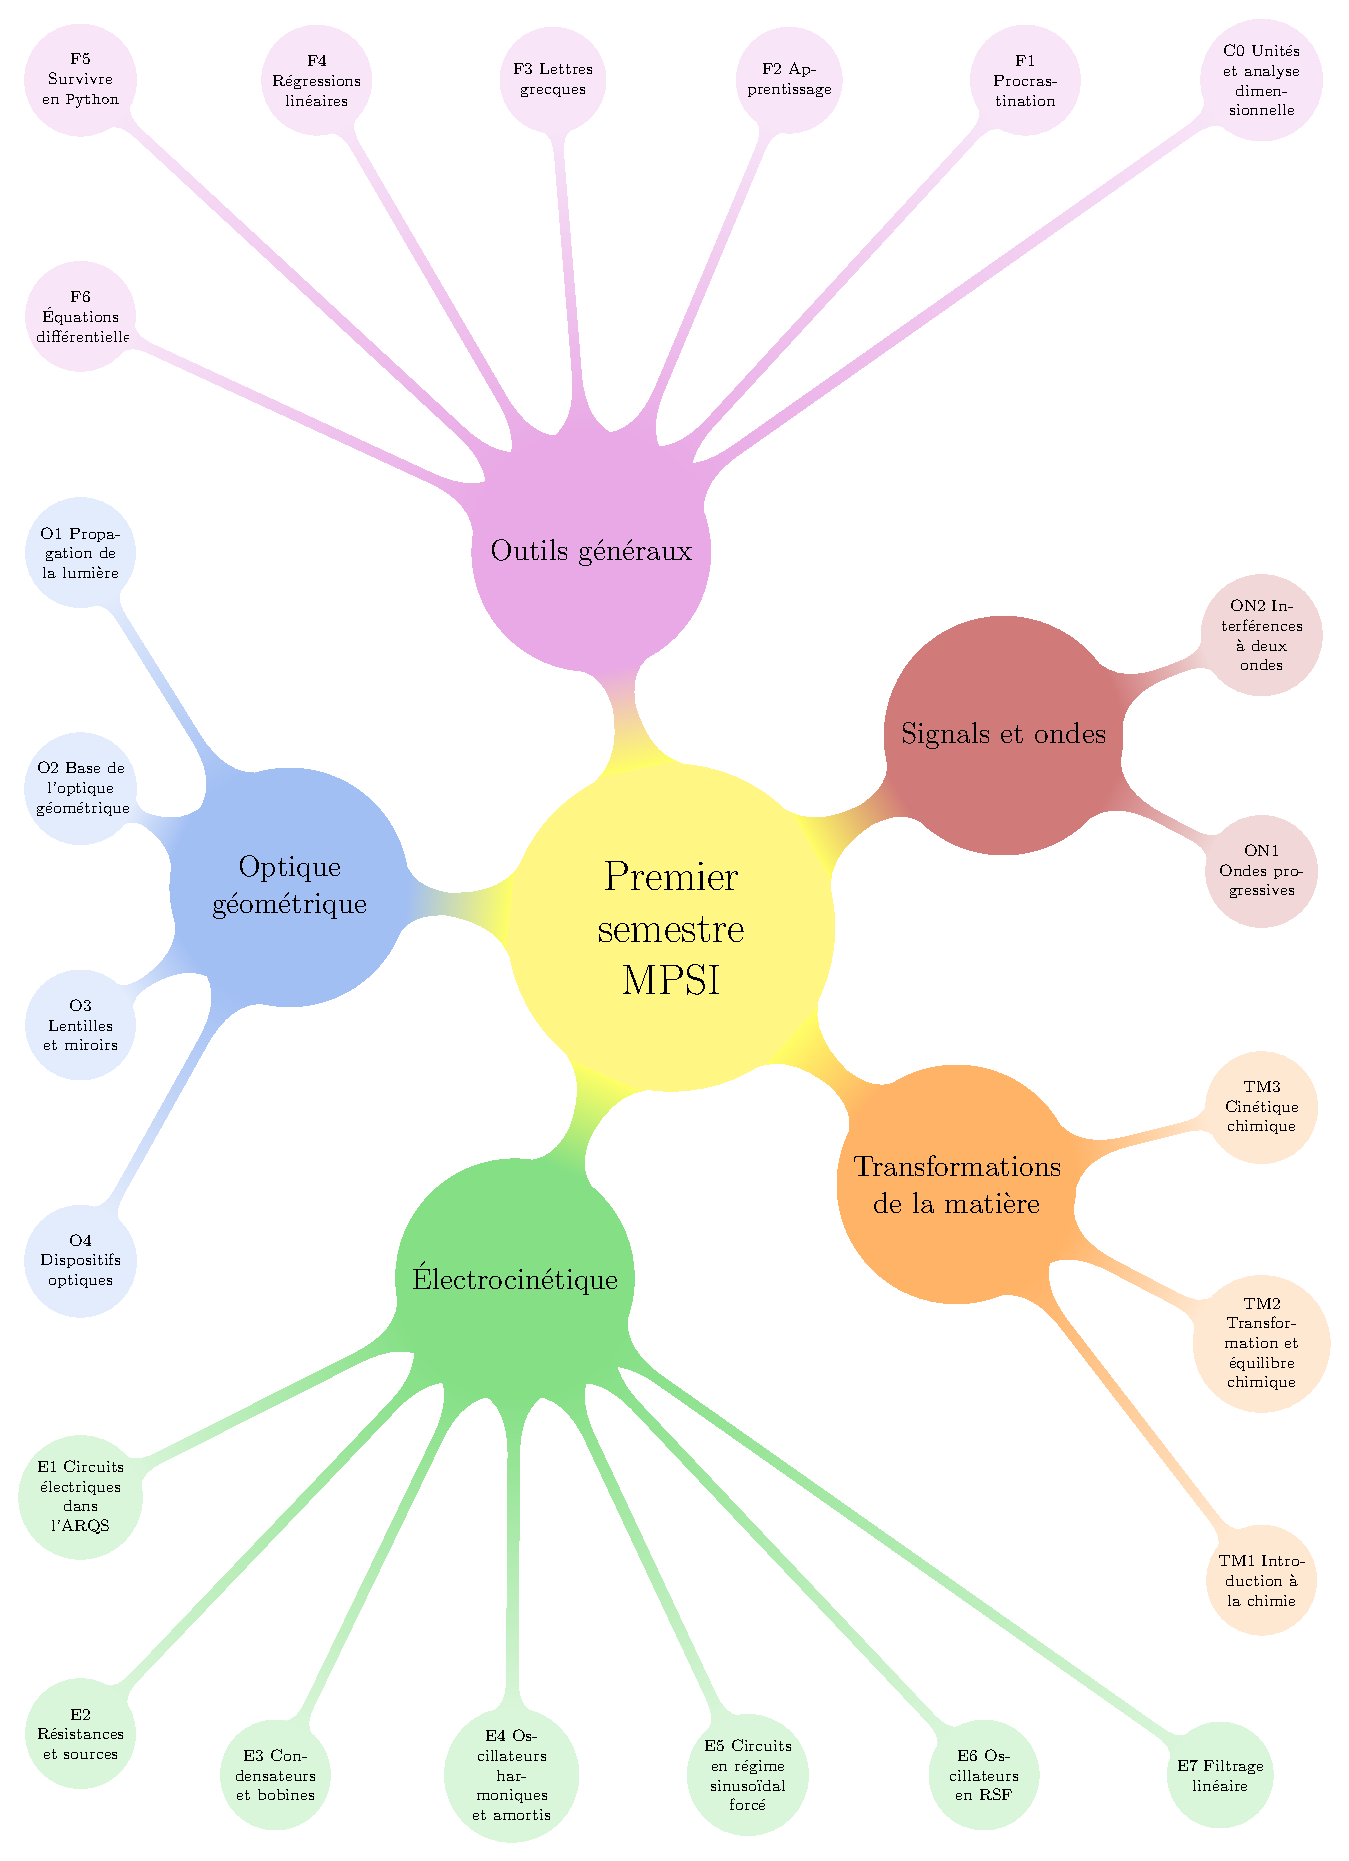
\includegraphics[width=\linewidth]{coverS1}
\end{adjustwidth}
\newpage

\tableofcontents
\listoffigures
\listoftables
\part{Outils généraux}
\subfile{../00_units/C0_units}
\subfile{../../00_Adm/Fiches/F00_organisation}
\subfile{../../00_Adm/Fiches/F01_procrastination}
% \subfile{../../00_Adm/Fiches/F02_apprentissage}
\subfile{../../00_Adm/Fiches/F03_grec}
\subfile{../../00_Adm/Fiches/F04_reglin}
\subfile{../../00_Adm/Fiches/F06_python_montecarlo}
\subfile{../../00_Adm/Fiches/F07_equa_diff}
\part{Optique géométrique}
\subfile{../01_optique/O1/O1_proplum}
\subfile{../01_optique/O2/O2_baseopt}
\subfile{../01_optique/O3/O3_mirlent}
\subfile{../01_optique/O4/O4_dispopt}
\part{Électrocinétique}
\subfile{../02_elec/E1/E1_cirarqs}
\subfile{../02_elec/E2/E2_ressourc}
\subfile{../02_elec/E3/E3_capaind}
\subfile{../02_elec/E4/E4_oscharmamor}
\subfile{../02_elec/E5/E5_rsf}
\subfile{../02_elec/E6/E6_oscrsf}
\subfile{../02_elec/E7/E7_filtrage}
\part{Transformations de la matière}
\subfile{../03_chimie/C1/C1_intro}
\subfile{../03_chimie/C2/C2_equi}
\subfile{../03_chimie/C3/C3_cine}
\part{Ondes}
\subfile{../04_ondes/ON1/ON1_ondesp}
\subfile{../04_ondes/ON2/ON2_inter}

\newpage
\begin{adjustwidth}{-1cm}{-1cm}
	\pagestyle{empty}
	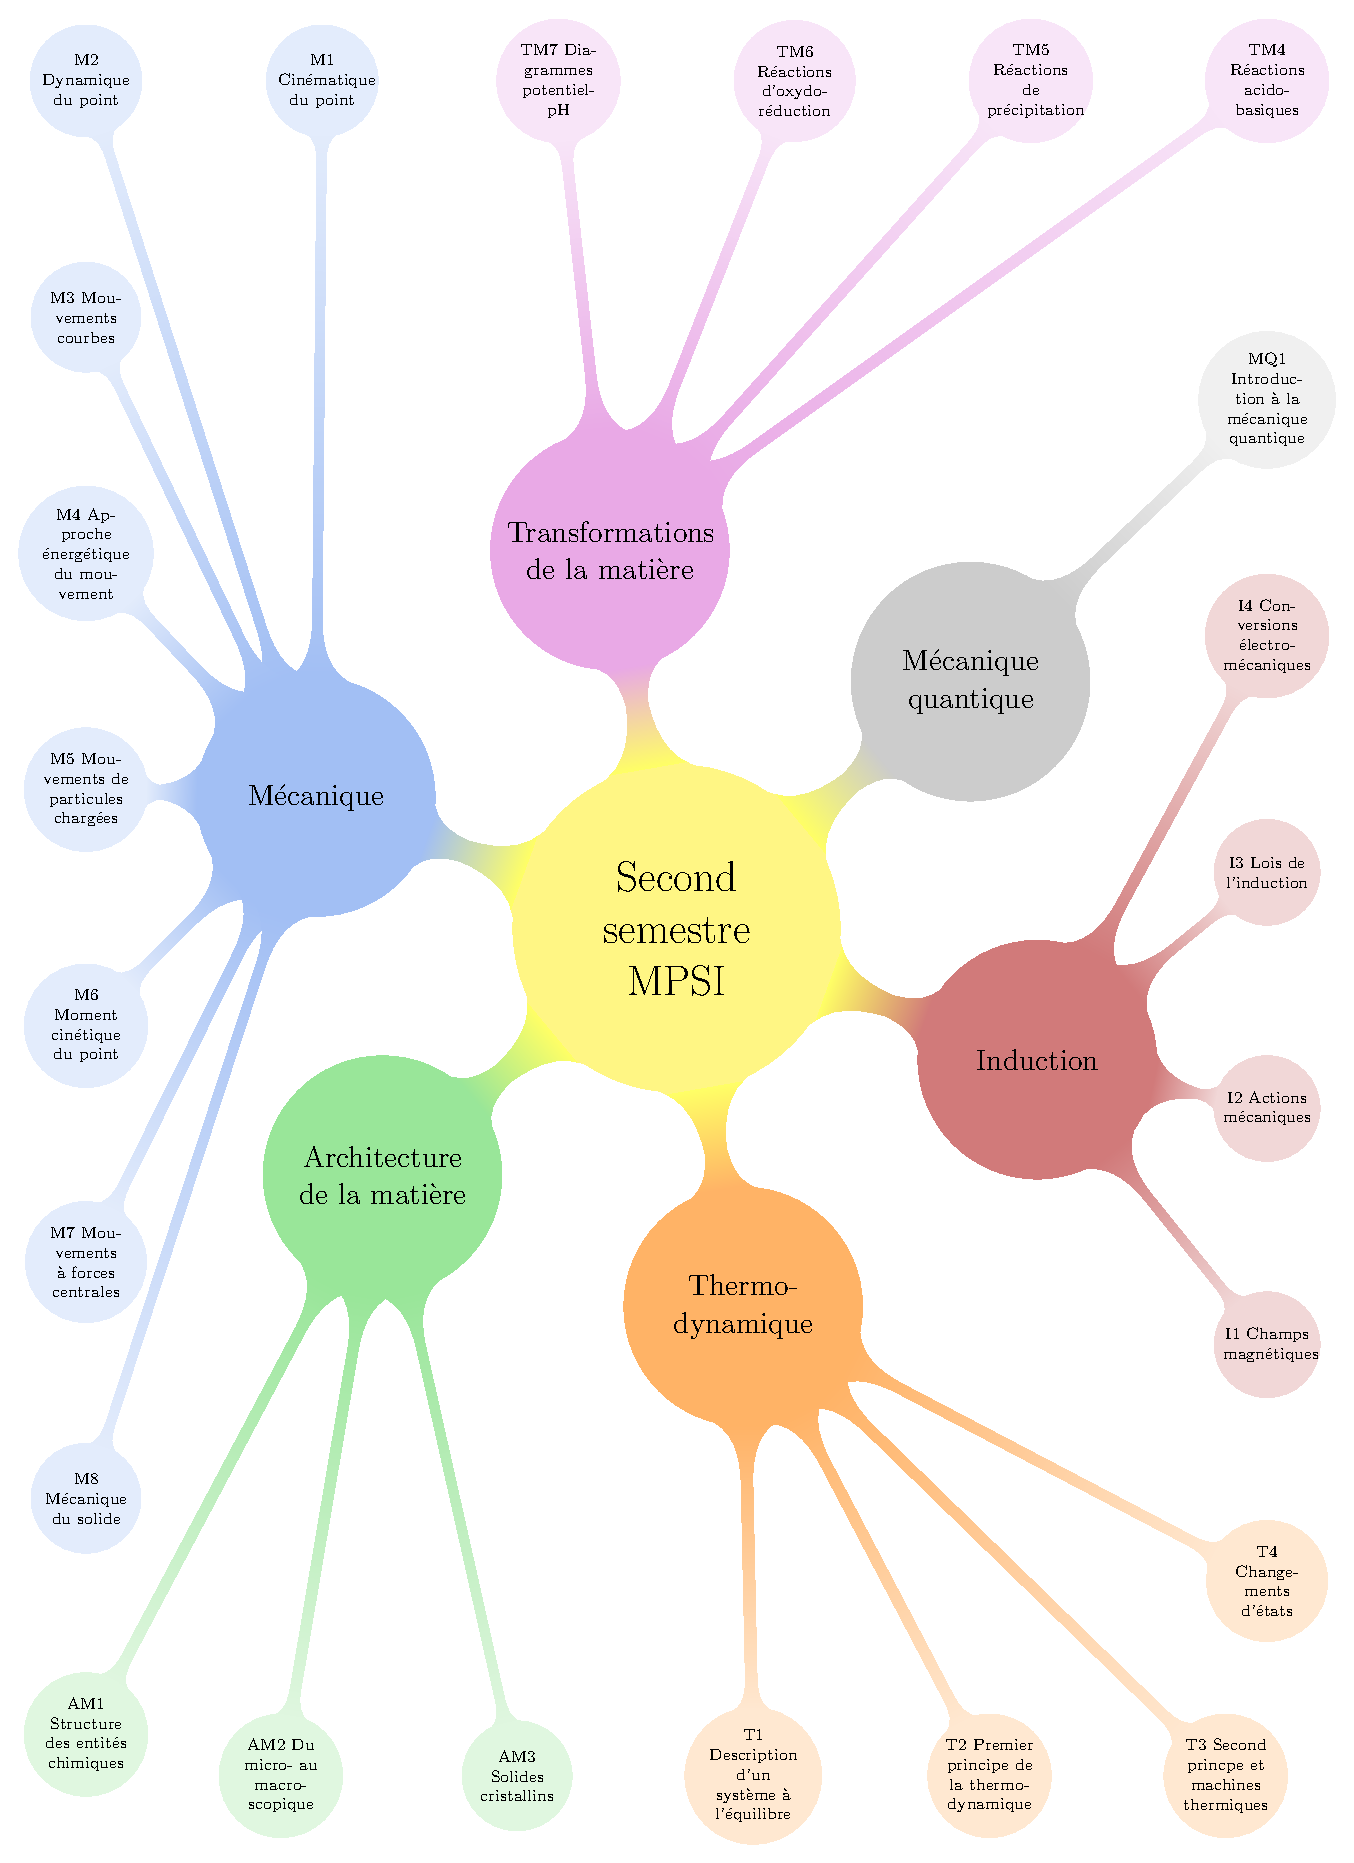
\includegraphics[width=\linewidth]{coverS2}
\end{adjustwidth}
\newpage
\part{Mécanique}
\subfile{../05_meca/M1/M1_cine}
\subfile{../05_meca/M2/M2_dyna}
\subfile{../05_meca/M3/M3_courbe}
\subfile{../05_meca/M4/M4_energ}
\subfile{../05_meca/M5/M5_charge}
\subfile{../05_meca/M6/M6_moment}
\subfile{../05_meca/M7/M7_central}
\subfile{../05_meca/M8/M8_solide}
\part{Architecture de la matière}
\subfile{../06_archmat/AM1/AM1_struc}
\subfile{../06_archmat/AM2/AM2_pptes}
\subfile{../06_archmat/AM3/AM3_cristallo}
\part{Transformations de la matière}
\subfile{../03_chimie/C4/C4_ab}
\subfile{../03_chimie/C5/C5_precip}
\subfile{../03_chimie/C6/C6_oxred}
\subfile{../03_chimie/C7/C7_eph}
\part{Thermodynamique}
\subfile{../07_thermo/T1/T1_desc}
\subfile{../07_thermo/T2/T2_preppe}
\subfile{../07_thermo/T3/T3_sndppemach}
\subfile{../07_thermo/T4/T4_etat}
\part{Induction}
\subfile{../08_induction/I1/I1_chpmag}
\subfile{../08_induction/I2/I2_actmag}
\subfile{../08_induction/I3/I3_neumann}
\subfile{../08_induction/I4/I4_conver}
\part{Mécanique quantique}
\subfile{../09_mq/MQ1/MQ1_intro}
% \bibliographystyle{../main/aa_url}
% \shorthandoff{:}
% \bibliography{../chapters/99_references}
\end{document}
